\documentclass{article}
\usepackage{tikz}
\usetikzlibrary{bbox}
\begin{document}
\subsection*{Without library}
\foreach \X in {1,...,40}
{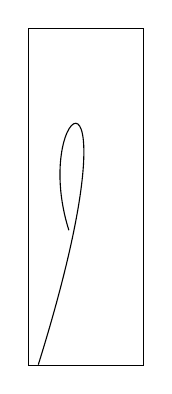
\begin{tikzpicture}
\draw (0,0)  .. controls (360*rnd:3*rnd) and (360*rnd:3*rnd) .. (360*rnd:3*rnd);
\draw (current bounding box.south west) rectangle 
  (current bounding box.north east);
\end{tikzpicture}\space}

\foreach \X in {1,...,40}
{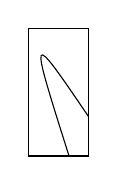
\begin{tikzpicture}
\draw (0,0)  .. controls (360*rnd:3*rnd) .. (360*rnd:3*rnd);
\draw (current bounding box.south west) rectangle 
  (current bounding box.north east);
\end{tikzpicture}\space}



\subsection*{With library}
\begingroup
\tikzset{bezier bounding box}
\foreach \X in {1,...,40}
{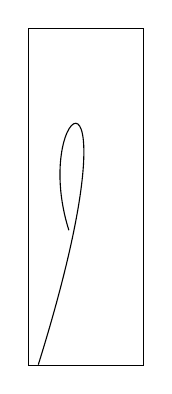
\begin{tikzpicture}
\draw (0,0)  .. controls (360*rnd:3*rnd) and (360*rnd:3*rnd) .. (360*rnd:3*rnd);
\draw (current bounding box.south west) rectangle 
  (current bounding box.north east);
\end{tikzpicture}\space}

\foreach \X in {1,...,40}
{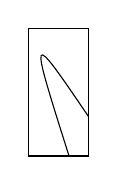
\begin{tikzpicture}
\draw (0,0)  .. controls (360*rnd:3*rnd) .. (360*rnd:3*rnd);
\draw (current bounding box.south west) rectangle 
  (current bounding box.north east);
\end{tikzpicture}\space}
\endgroup
\end{document}
